\section{VideoMix}
\label{section:videomix}

In this section, we analyze existing data augmentations, describe the VideoMix algorithm, and discuss the effectiveness of VideoMix. 

\subsection{Revisiting Data Augmentation Techniques}

\begin{table}[t]
\centering
\begin{tabular}{@{}lccc@{}}
\toprule
Methods              & top1  & top5  \\ \midrule
Vanilla      &   75.2 &  91.7    \\
Mixup~\cite{zhang2017mixup}         &   77.0 &  93.1     \\
RandAugment~\cite{randaugment}   &   75.6 &   92.2    \\ 
Cutout~\cite{devries2017cutout}        &   76.1 &  92.6      \\
CutMix~\cite{cutmix}      &  76.7    &  92.9     \\  
\midrule
VideoMix       &  \textbf{77.6}    &  \textbf{93.5} \\
\midrule
\end{tabular}
\caption{\textbf{VideoMix vs existing data augmentation techniques.} The compared baselines are originally proposed for the image classification tasks. We extend them from two spatial dimensions to three spatio-temporal dimensions. SlowOnly-34 ($8\times8$) network and Mini-Kinetics dataset are used. 
}
\label{table:method:analysis}
\end{table}




We review existing data augmentation methods that partially remove regions in an image~\cite{devries2017cutout}, add pixel-level noises~\cite{autoaugment,randaugment}, or manipulate both input pixels and labels~\cite{zhang2017mixup,cutmix}.
We first evaluate their effectiveness by simply extending the two-dimensional methods to the three spatio-temporal dimensions.

Table~\ref{table:method:analysis} compares the augmentation strategies including Mixup~\cite{zhang2017mixup}, RandAugment~\cite{randaugment}, Cutout~\cite{devries2017cutout}, and CutMix~\cite{cutmix}.
It is straightforward to extend Mixup and RandAugment to videos: they apply global operations over the pixels. Mixup averages the RGB values of two images and RandAugment applies rotation, shear, and uniform perturbations on the images. We apply the same operation over the spatio-temporal frames.
For Cutout and CutMix, we choose the full spatio-temporal extension where sub-cuboids in videos are randomly selected to be removed or replaced.
We set the hyperparameter $\alpha$ of Mixup and CutMix to $1.0$, the mask size for Cutout to $112\times112$, the magnitudes $M$ for RandAugment to $9$.
Table~\ref{table:method:analysis} shows that even the naive extension of the baselines lead to improvements in video classification against the vanilla model. For example, Mixup achieves 77.0\% top-1 accuracy on Mini-Kinetics, an $+\mathbf{1.8}\%$ improvement against the vanilla SlowOnly-34 ($8\times8$) model.

In the rest of the section, we seek ways to boost the video recognition performances further by studying the design choices in augmentation strategies in greater depth.


\subsection{VideoMix Algorithm}
\label{section:videomix:algorithm}
We introduce the \textbf{VideoMix} algorithm.
Let $x \in \mathbb{R}^{T \times W \times H}$ be a video sequence, where $T$, $W$, and $H$ are the number of frames, width, and height of video sequences, respectively\footnote{We omit the input channel dimension (3 for RGB) for simplicity.}. Let $y$ be the corresponding ground truth label, represented as a one-hot vector. 
VideoMix generates a new training sample $(\Tilde{x},\Tilde{y})$ by combining two training samples $(x_{A}, y_{A})$ and $(x_{B}, y_{B})$. 
The generated $(\Tilde{x},\Tilde{y})$ is used for training the model with its original loss function.

More precisely, VideoMix first defines a binary tensor mask $\mathbf{M} \in \{0,1\}^{T \times W \times H}$ signifying the cut-and-paste locations in two video tensors. The new video is generated by the below procedure:
\begin{equation}
\begin{split}
    \Tilde{x} & =  \mathbf{M} \odot x_{A} + (\mathbf{1}- \mathbf{M}) \odot x_{B} \\
    \Tilde{y} & =  \lambda_\mathbf{M} y_A + (1-\lambda_\mathbf{M}) y_B
\end{split}
\label{eq:cutmix}
\end{equation}
where $\odot$ is the element-wise multiplication and $\lambda_\mathbf{M} := \frac{1}{TWH}\sum_{t,w,h}\mathbf{M}_{t,w,h}$
denotes the proportion of the volume occupied by $\mathbf{M}$.

The binary tensor mask $\mathbf{M}$ is decided by drawing the 3D cuboid coordinates $\mathbf{C}=(t_1,t_2,w_1,w_2,h_1,h_2)$ at random. More specifically,
\begin{align}
\small
    \mathbf{M}_{t,w,h}:=
    \begin{cases}
        1,&\text{ if }\quad t_1\leq t \leq t_2\text{, }w_1\leq w \leq w_2\text{, and } h_1\leq h \leq h_2 \\
        0,&\text{ otherwise}
    \end{cases}
\end{align}
We will investigate the design choices for the random selection of coordinates in the next part.


\subsection{Investigation of spatial and temporal axes for VideoMix}
\begin{figure}[!t]
\centering
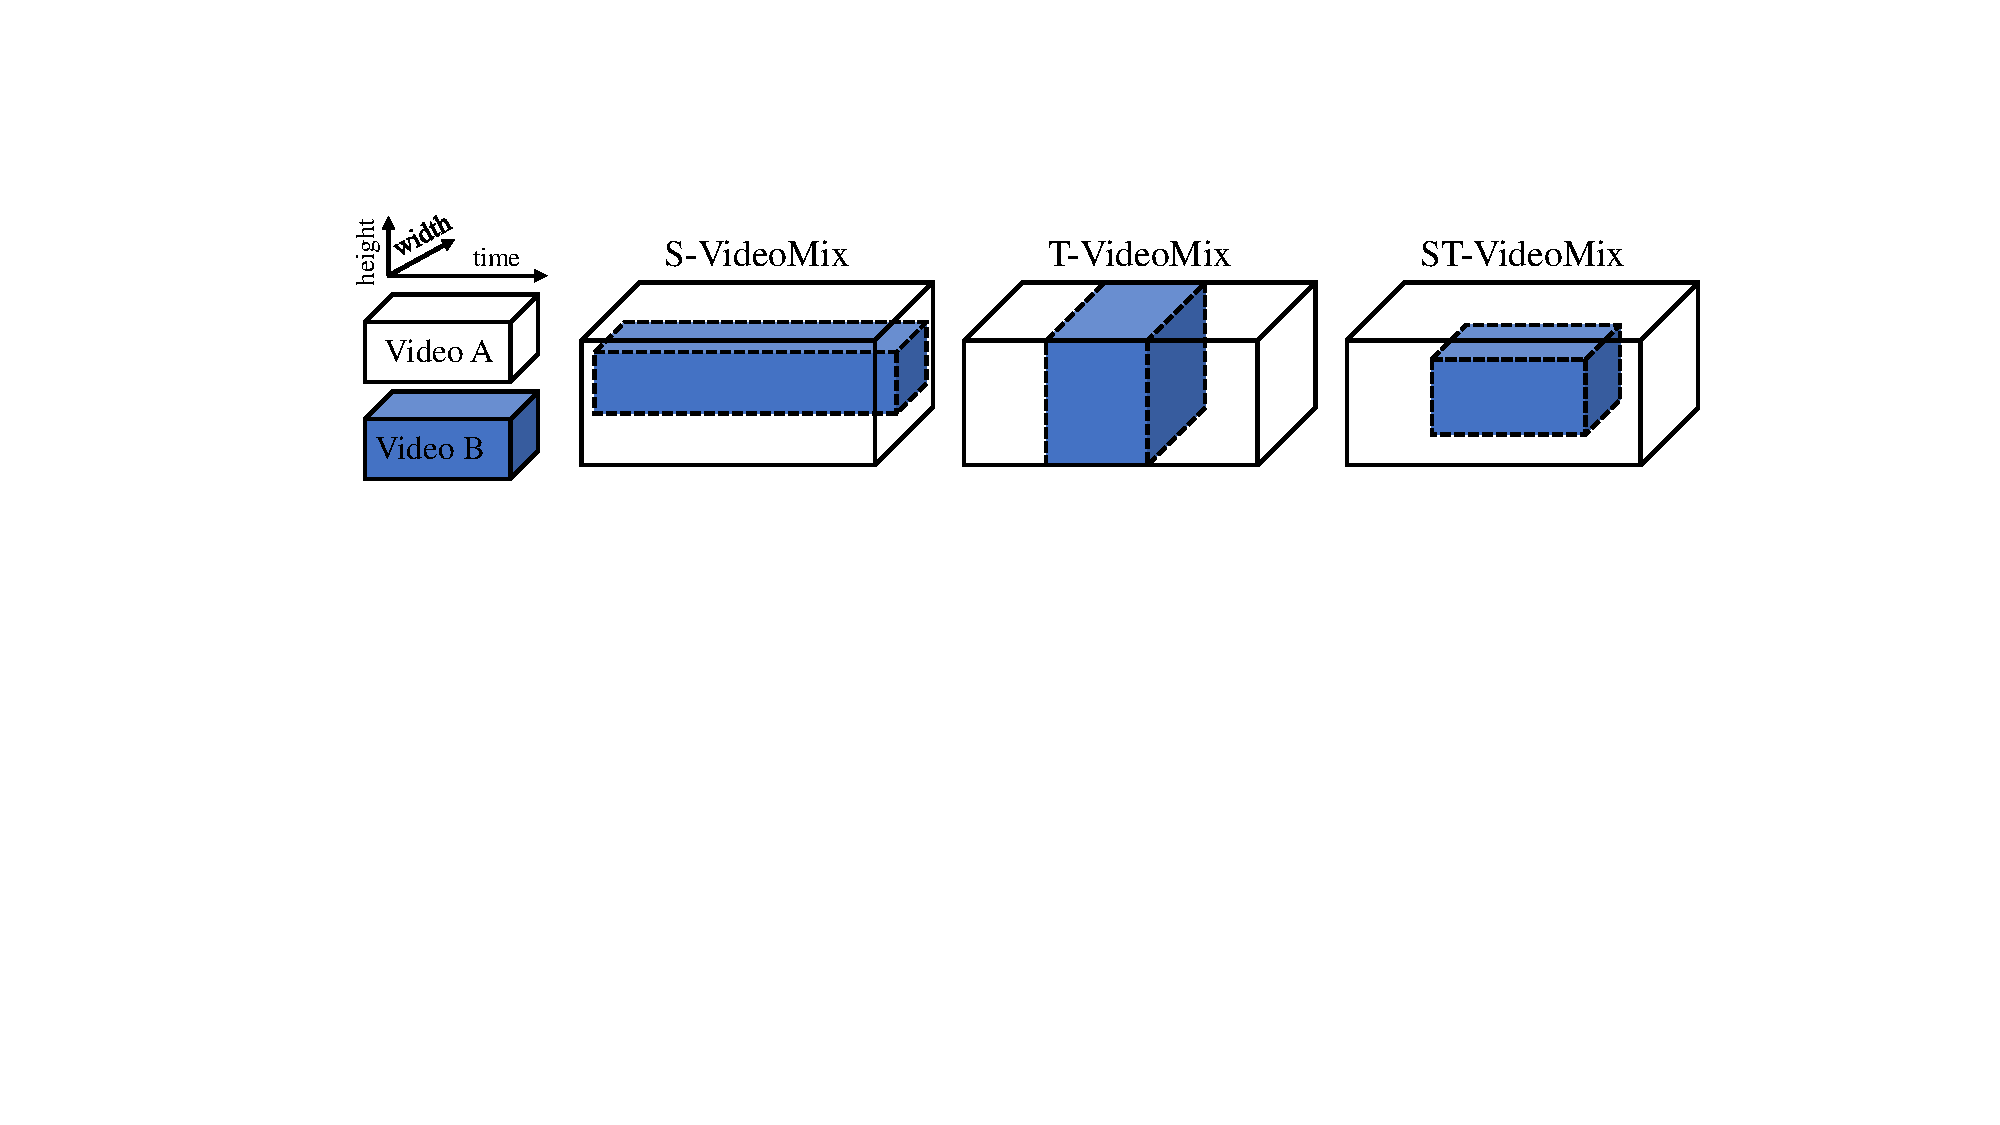
\includegraphics[width=\linewidth]{arxiv_videomix/main/figures/videomix.pdf}
\caption{\textbf{VideoMix variants.} Illustrations of Spatial (S-), Temporal (T-), and Spatio-temporal (ST-) VideoMix. 
We omit the channel (color) dimension for clarity. A sub-cuboid of Video B (blue cube) is inserted into Video A (white cube).}
\label{fig:videomix:videomix_types}
\end{figure}
\begin{table}[!t]
\centering
\begin{tabular}{@{}lccc@{}}
\toprule
Methods              & top1  & top5  \\ \midrule
Spatial VideoMix       &  \textbf{77.6}    &  \textbf{93.5} \\
Temporal VideoMix       &   75.6   & 92.5 \\
Spatio-temporal VideoMix       & 76.7  & 92.9\\
\midrule
\end{tabular}
\caption{\textbf{Performances of VideoMix variants.} Performances of Spatial, Temporal, and Spatio-temporal VideoMix. SlowOnly-34 ($8\times8$) network and Mini-Kinetics dataset are used.
}
\label{table:method:videomix_types}
\end{table}

We identify three types of VideoMix: Temporal, Spatial, and Spatio-temporal VideoMix.
Temporal VideoMix samples the cuboid coordinates $\mathbf{C}$ only along the temporal axis ($(t_1,t_2)$ are sampled) and fixes spatial coordinates at $(w_1,w_2,h_0,h_1)=(0,W,0,H)$. Spatial VideoMix samples the spatial coordinates $(w_1,w_2,h_1,h_2)$, while fixing $(t_1,t_2)=(0,T)$. 
Spatio-temporal VideoMix samples all the coordinates $(t_1,t_2,w_1,w_2,h_1,h_2)$.
The VideoMix variants are illustrated in Figure~\ref{fig:videomix:videomix_types}. 
Note that the Spatio-temporal VideoMix is the same as the CutMix in Table~\ref{table:method:analysis}.

Table~\ref{table:method:videomix_types} compares the performances of the VideoMix variants. Spatial VideoMix is the best among them. We hypothesize that the video sub-cuboid must secure a sufficient number of frames to represent the semantic information for the video category. Temporal VideoMix or Spatio-temporal VideoMix is limited in terms of the semantic content in cut and pasted video cuboids.
Spatial VideoMix, on the contrary, retains the full temporal semantics.

Based on this observation, we define \textbf{Spatial VideoMix} as our default VideoMix setting for video classification task.
The random coordinate selection strategy follows that of CutMix~\cite{cutmix}.
The spatial ratio $\lambda$ is sampled from the Beta distribution Beta($\alpha$,$\alpha$), where we set $\alpha:=1$\footnote{When $\alpha=1$, it is the uniform distribution $\text{Unif}(0,1)$.}.
The center coordinates $(w_c,h_c)$ are sampled from $\text{Unif}(0,W)\times\text{Unif}(0,H)$. Other cuboid endpoints are determined by 
\begin{equation}
\begin{split}
    w_{1} = w_c - \frac{W\sqrt{\lambda}}{2}~~~ & w_{2} = w_c + \frac{W\sqrt{\lambda}}{2} \\
    h_{1} = h_c - \frac{H\sqrt{\lambda}}{2}~~~ & h_{2} = h_c + \frac{H\sqrt{\lambda}}{2}
\end{split}
\label{eq:sampling}
\end{equation}
and fixed $(t_1,t_2)=(0,T)$.
Codes for VideoMix variants are presented in Appendix~\ref{appendix:algorithm}. 

\paragraph{VideoMix for temporal localization.}
Under certain application scenarios, it is difficult to directly manipulate the input videos. For example, features may have already been extracted from the original frames and the raw frames are unavailable because of the storage limits or legal issues~\cite{abu2016youtube}. 
As we will cover in the experiments of temporal action localization, \textbf{Temporal VideoMix} is a good alternative that improves the localization ability of a video classifier. 



\begin{figure}[!t]
\centering
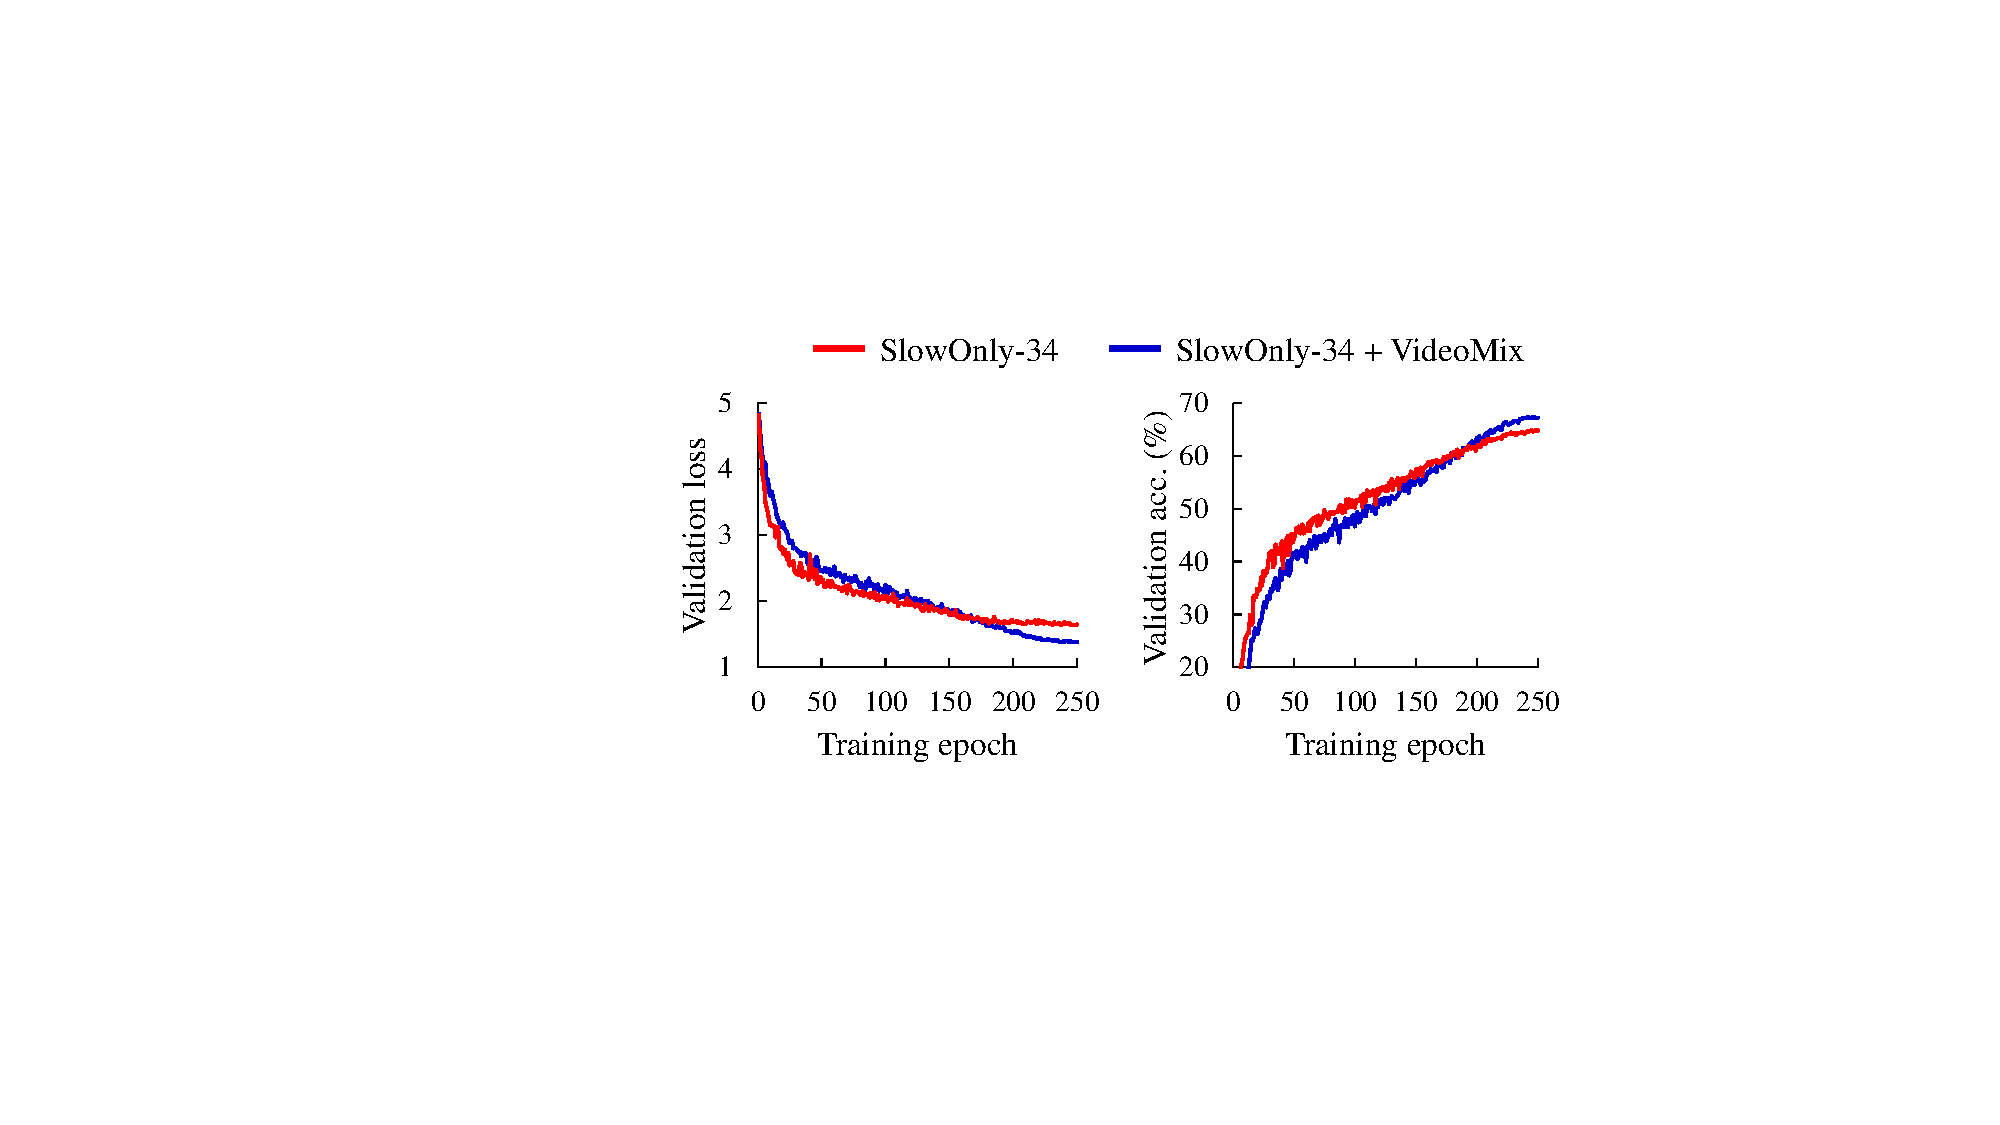
\includegraphics[width=\linewidth]{arxiv_videomix/main/figures/valloss.pdf}
\caption{\textbf{Training curves.} Validation loss (left) and top-1 accuracy (right) plots for Mini-Kinetics action recognition. VideoMix achieves lower validation loss and higher top-1 accuracy than the vanilla model.}
\label{fig:videomix:loss_plot}
\end{figure}



\subsection{Discussion}

\paragraph{Effect on preventing overfitting.}

To see the effect of VideoMix on preventing overfitting and stabilizing the training process, we compare validation loss and validation accuracy of SlowOnly-34 models during the training over Mini-Kinetics action recognition dataset in 
Figure~\ref{fig:videomix:loss_plot}.
We confirm that VideoMix enables video models to obtain lower validation loss and higher validation accuracy than the baseline. 
After about 200 training epochs, the baseline performance saturates and the loss does not decrease further.
Applying VideoMix lets the model overcome the barrier and improve further beyond this point. The training samples generated by VideoMix allow the video classifiers to generalize better.

\begin{figure*}[!t]
\centering
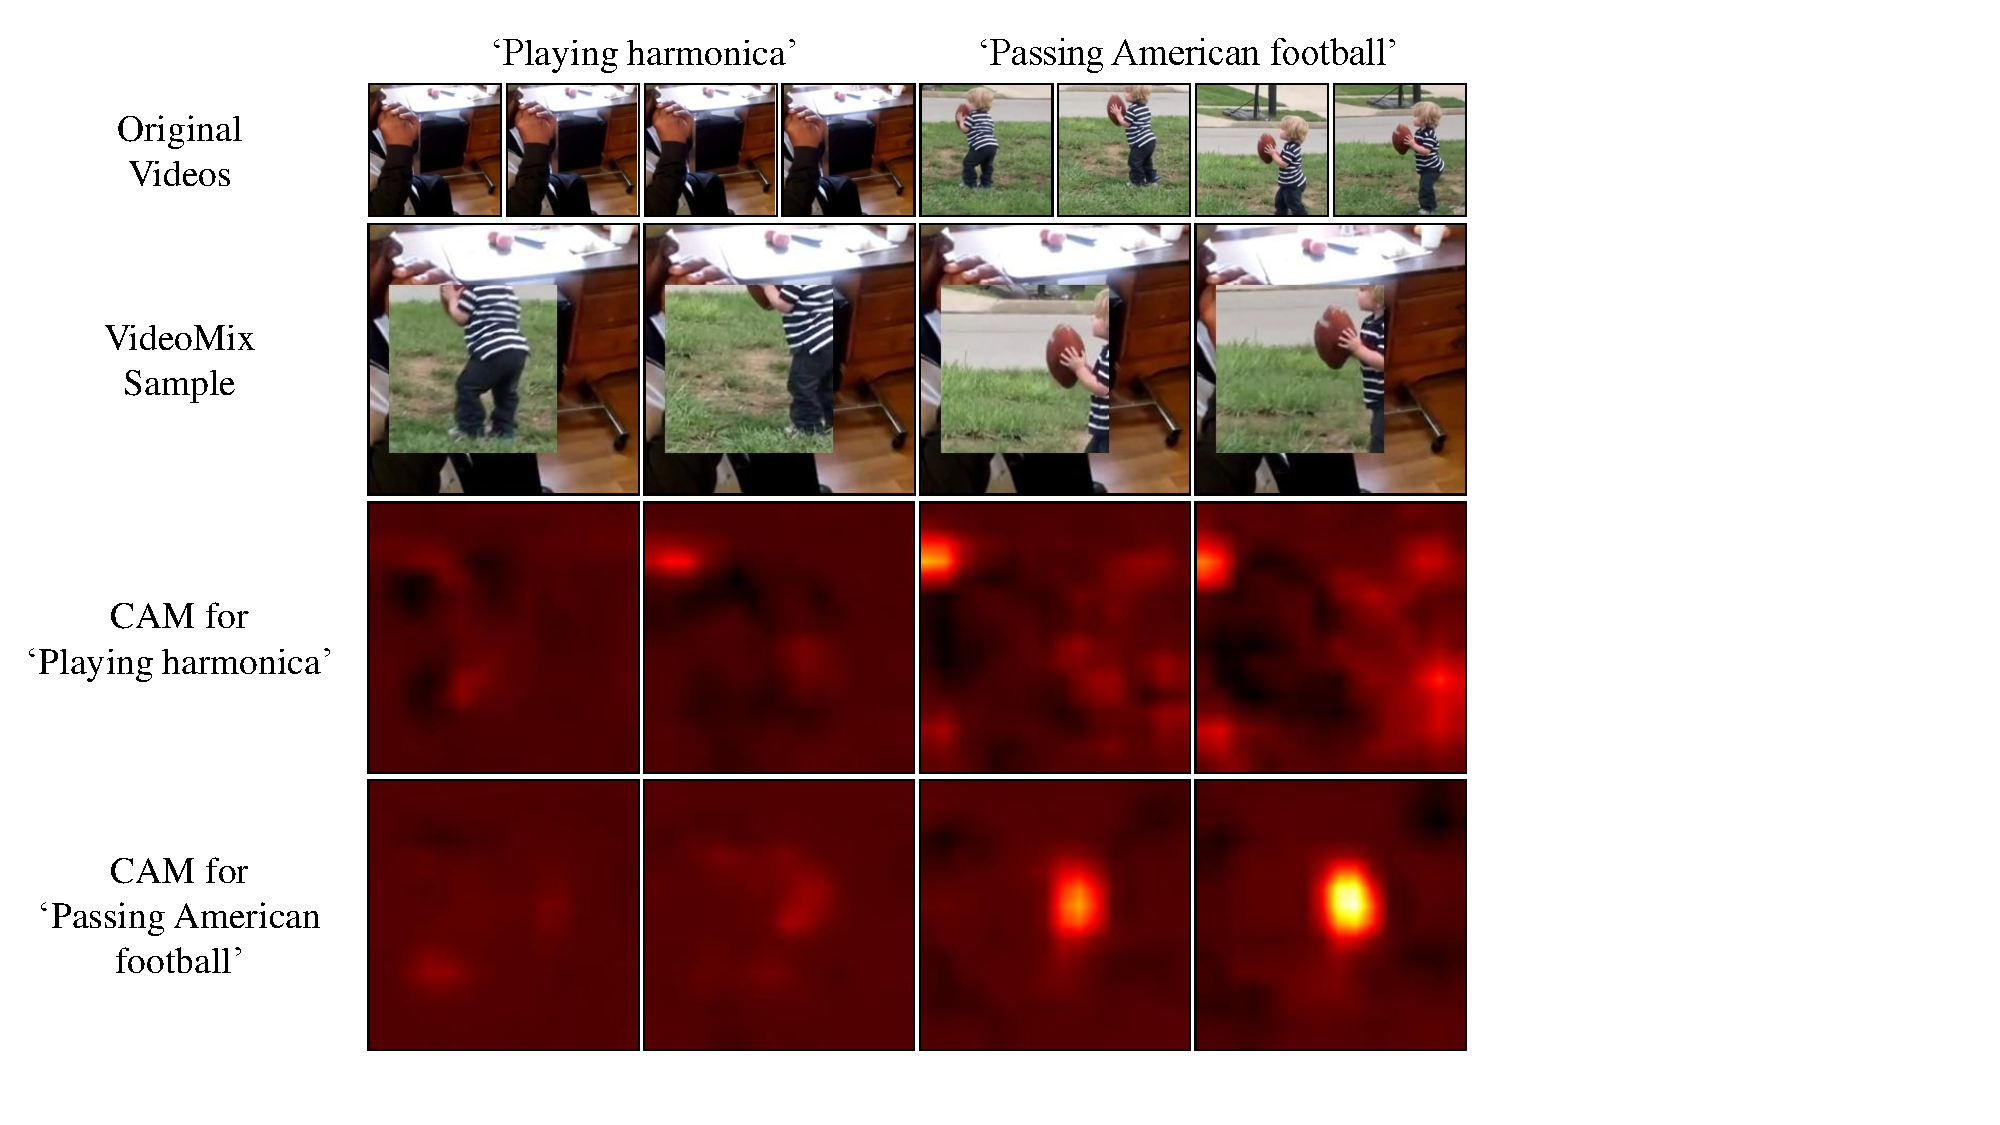
\includegraphics[width=0.80\linewidth]{arxiv_videomix/main/figures/cam2.pdf}
\caption{\textbf{Class activation mapping (CAM) on VideoMix sample.} We show the spatio-temporal CAM~\cite{zhou2016CAM} score maps on a VideoMix sample. It is a combination of the ``playing harmonica'' and ``passing American football'' videos. The CAM score maps are visualized with respect to the two action classes separately. 
}
\label{fig:videomix:cam_visualize}
\end{figure*}


\paragraph{What does the model learn with VideoMix?}

We expect VideoMix to let an action classifier simultaneously recognize multiple actions present in the mixed videos. To verify that this is achieved, we visualize the spatio-temporal attention of a video on the synthetic video generated by VideoMix with the class activation maps (CAM)~\cite{zhou2016CAM}.
We use a Kinetics-400 pre-trained SlowOnly-50 model. 
We extend the original CAM proposed for static images to its spatio-temporal version that generates the $T$ sequential score maps. 
Detail description of spatio-temporal CAM and more examples are in Appendix~\ref{appendix:algorithm}. 
Figure~\ref{fig:videomix:cam_visualize} shows VideoMix samples and corresponding class activation maps with respect to the two action classes, ``playing harmonica'' and ``passing American football''.
The CAM results show that VideoMix guides a model to see multiple actions at once (e.g., the CAM for ``playing harmonica'' highlights the player's mouth and hands, and the CAM for ``passing American football'' emphasizes the kid's hands and the football object).
Furthermore, VideoMix reduces scene contexts of videos, as the background scene of ``passing American football'' are partially removed, and also hides some object cues, as the football 
of ``passing American football'' and the hands holding a harmonica of ``playing harmonica'' are blocked in some frames, which leads to learning more robust and generalized cues beyond the object and scene for action recognition. 

